\documentclass{beamer}
\usetheme{Madrid}
\useinnertheme{rounded}
\usecolortheme{whale}

\title{Next Reaction Method}
\subtitle{Efficient Stochastic Simulation of Chemical Systems}
\author{Lorenzo Beretta}
\date{29th July 2019}

%pacchetti scrittura
\usepackage{dsfont}
\usepackage{amsthm}
\usepackage{amsmath}
\usepackage{amssymb}
\usepackage{mathrsfs}
\usepackage{mathtools}
\usepackage{enumitem}
\usepackage{hyperref}
\usepackage{marginnote}
\usepackage{scalerel}
\usepackage{comment}
\usepackage[utf8]{inputenc}

%% miei %%
\usepackage{tkz-graph}
\usepackage{algorithm,algorithmic}
\usepackage{tikz}
\usepackage{color}
\usepackage{centernot}
\usepackage{esvect}

% tikz
\usetikzlibrary{positioning,chains,fit,shapes,calc}
\definecolor{myblue}{RGB}{80,80,160}
\definecolor{mygreen}{RGB}{80,160,80}


\begin{document}

\begin{frame}
  \maketitle
\end{frame}

\begin{frame}{Predictive Model Definition}
  To define a predictive model we need two steps:
  \begin{itemize}
  \item $\bullet$ Define a descriptive model of the phenomenon
    \begin{block}{Descriptive Model: Differential Equation}
      The Newton's law of motion:
      $$ \vv{F} = m \, \frac{\partial^2 \vv{x}}{\partial t^2} $$
    \end{block}
    
  \item $\bullet$ Define a computational model to make predictions
    \begin{block}{Computational Model: Numerical Integration}
      \begin{figure}[h]
        \centering
        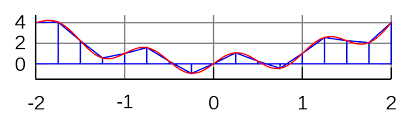
\includegraphics[scale=0.6]{num_int}
      \end{figure}

    \end{block}

  \end{itemize}
\end{frame}

\begin{frame}{Descriptive Model Definition}
	\begin{block}{Torneo}
	$T=\left(V,A\right)$ un grafo diretto e completo.
	\end{block}
	\begin{center}
		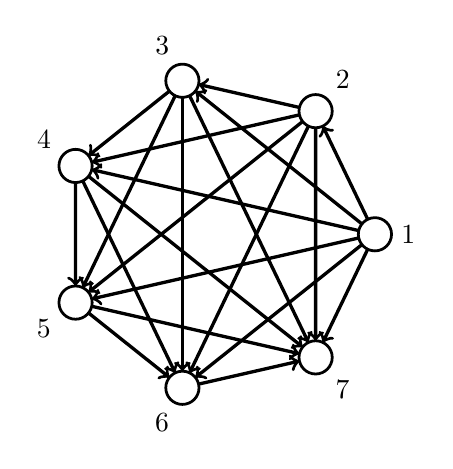
\begin{tikzpicture}
			\SetGraphUnit{2}
			\renewcommand*{\VertexLineColor}{black}
			\renewcommand*{\VertexLightFillColor}{white}
			\renewcommand*{\VertexLineWidth}{1pt}
			\GraphInit[vstyle=Welsh]
			\Vertices{circle}{1,2,3,4,5,6,7}
			\SetUpEdge[style={->, very thick}, color=black]
			\foreach \v in {1,...,5,6} {
				\foreach \vv in {\v,...,6,7} {
					\ifthenelse{\v=\vv} {} {
						\Edge(\v)(\vv)
					}
				}
			}
		\end{tikzpicture}
	\end{center}
\end{frame}

\begin{frame}{Matrice di adiacenza di un Torneo}
	\begin{columns}
		\begin{column}{.5 \textwidth}
			\[
			A = \begin{bmatrix}
				0 & 1 & 0 & 0 & 1 & 1 & 0 \\
				0 & 0 & 1 & 1 & 0 & 0 & 0 \\
				1 & 0 & 0 & 1 & 0 & 1 & 0 \\
				1 & 0 & 0 & 0 & 0 & 0 & 1 \\
				0 & 1 & 1 & 1 & 0 & 0 & 1 \\
				0 & 1 & 0 & 1 & 1 & 0 & 0 \\
				1 & 1 & 1 & 0 & 0 & 1 & 0 \\
		    \end{bmatrix}
			\]
		\end{column}

		\begin{column}{.5 \textwidth}
			\begin{block}{Definizioni}
				\vspace{2mm}
				$\bullet$ $ A_{i,j} = 1 \iff i \longrightarrow j \text{ in } T $ \\
				\vspace{2mm}
				$\bullet$ $ A_{i,j} + A_{j, i} = 1 $ \\
				\vspace{2mm}
				$\bullet$ $ d^+(i) = \sum\limits_{j = 1}^n A_{i, j} $ \\
				\vspace{2mm}
				$\bullet$ $ d^-(i) = n - 1 - d^+(i) $ \\
				\vspace{2mm}
			\end{block}
		\end{column}
	\end{columns}
\end{frame}

\begin{frame}{Contesto}
	Direzioni della letteratura esistente:
	\vspace{3mm}
		\begin{itemize}
			\item  $\bullet$ Proprietà combinatorie:
			\begin{center}
				\begin{minipage}{.7 \textwidth}
					\begin{block}{Congettura di Kelly}
						Gli archi di un $n$-torneo, per $n$ pari, si possono partizionare in $\frac{n-1}{2}$ cicli Hamiltoniani.
					\end{block}
				\end{minipage}
			\end{center}
			\begin{center}
				\begin{minipage}{.7 \textwidth}
					\begin{block}{Congettura di Sumner}
						Un $(2n-2)$-torneo contiene ogni orientamento di ogni $n$-albero.
					\end{block}
				\end{minipage}
			\end{center}

		\pause
			\item $\bullet$ Applicazioni:
			\begin{itemize}
				\vspace{3mm}
				\item Esperimenti a coppie
				\vspace{3mm}
				\item Teoria del Voto
			\end{itemize}

	\end{itemize}
\end{frame}

\begin{frame}{Problema: trovare il campione}
	\begin{block}{Definizione di Campione}
		Possibili metriche:
		\begin{itemize}
			\item $\bullet$ Minimum FAS (feedback arc set)
			\item $\bullet$ King
			\item $\bullet$ MOD (Maximum out-degree)
		\end{itemize}
	\end{block}
	\pause
	\begin{block}{Minimum FAS}
		Trovare $\left(V, \prec\right)$ che minimizzi
		$$ \# \left\{i \prec j \; | \; i \longrightarrow j \right\} $$
		Complessità: $\mathcal{NP}$-hard \\
		\vspace{3mm}
		Ha molte buone proprietà ma è irrealizabile
	\end{block}
\end{frame}

\begin{frame}{Problema: trovare il campione}
	\begin{block}{King}
		Trovare $x \in V $ tale che $\forall y \in V$
		$$ x \longrightarrow y \quad \text{o} \quad \exists w \in V \quad \text{t.c.} \quad x \longrightarrow w \quad \text{e} \quad w \longrightarrow y $$
		Complessità: $O\left(n\right)$ \\
		\pause
		\begin{center}
			\begin{minipage}{.7 \textwidth}
				\begin{block}{Teorema}
					In quasi ogni torneo ogni vertice è un King.
				\end{block}
			\end{minipage}
		\end{center}
		Facile da computare ma scarse proprietà
	\end{block}
\end{frame}

\begin{frame}{Problema: trovare il campione}
	\begin{block}{MOD (Maximum out-degree)}
		Trovare $ x \in V$ che massimizzi il numero di partite vinte $d^+\left(x\right)$ \\
		\vspace{3mm}
		Complessità: $\Theta\left(n^2\right)$ \\
		\begin{center}
			MOD $\implies$ King \\
			\vspace{3mm}
			min FAS $\centernot\implies$ MOD \\
		\end{center}
	\end{block}
	\pause
	\begin{block}{Complessità: Dimostrazione}
		L'algoritmo brute force ci dà $O\left(n^2\right)$ \\
		\vspace{3mm}
		Mostriamo che nel worst case otteniamo $\Omega\left(n^2\right)$
		\vspace{3mm}
	\end{block}
\end{frame}

\begin{frame}{MOD: Complessità}
	\begin{block}{Dimostrazione}
		Tratteremo il caso $n$ dispari, consideriamo $T$ \textit{regolare}, ovvero
		$$ \forall x \in V \quad d^+(x) = \frac{n-1}{2} $$
		\pause
		\begin{center}
			\begin{minipage}{.7 \textwidth}
				\begin{block}{Definizioni}
					\begin{itemize}
						\item $\bullet$ $S \subseteq V^2$ archi scoperti
						\item $\bullet$ $\pi_i(S) = \left\{j \in S \big| (i, j) \in S \right\}$
					\end{itemize}
				\end{block}
			\end{minipage}
		\end{center}

		% Sia $y$ il vincitore trovato, necessariamente $d^+(y) = \frac{n-1}{2}$ \\
		% \vspace{3mm}
		\pause
		Se $\exists w \in V\;$ t.c. $\left|\pi_w(S)\right| < \frac{n-1}{2}\;$ allora posso renderlo il campione \\
		\vspace{3mm}
		Se $\forall w \in V \quad \left|\pi_w(S)\right| \geq \frac{n-1}{2} \implies \left|S\right| \geq \frac{(n-1)^2}{2}$
	\end{block}
\end{frame}

\begin{frame}{MOD: Oracolo Impreciso}
	\begin{block}{Oracolo Impreciso}
		Consideriamo il torneo prodotto da un oracolo impreciso \\
		\vspace{3mm}
		Nell'applicazione questo è un algoritmo di ML imperfetto ma efficace \\
		\vspace{3mm}
		Possiamo quindi parametrizzare la complessità rispetto a $\ell = \min\limits_{i \in V} \:d^-\left(i\right)$ \\
	\end{block}
	\pause
	\begin{block}{Nuovo Lower Bound}
		$$ \Omega\left(\ell n\right) $$

		infatti se effettuiamo $o(\ell n)$ lookup allora:
		$$ \exists i \text{ t.c. } \big|\pi_i(S)\big| < \ell $$
		possiamo completare il torneo in modo che $ d^-(i) < \ell $

	\end{block}

\end{frame}

\begin{frame}{MOD: Algoritmo}
	\begin{columns}
		\begin{column}{.5 \textwidth}
			\begin{algorithm}[H]
				\begin{algorithmic}[1]
					\WHILE {$\forall i \;\: \pi_i\left(S\right) \neq V$}
						\FOR {$i = 1, .., n$}
							\STATE {$r = Rand\left(V \setminus \pi_i\left(S\right)\right)$}
							\STATE {$S = S \cup \left\{\left(i, r \right)\right\}$}
							\WHILE {$i \longrightarrow r$}
								\STATE {$r = Rand\left(V \setminus \pi_i\left(S\right)\right)$}
								\STATE {$S = S \cup \left\{\left(i, r \right)\right\}$}
							\ENDWHILE
						\ENDFOR
					\ENDWHILE
				\end{algorithmic}
			\end{algorithm}
		\end{column}
		\begin{column}{.5 \textwidth}
			\[
			\begin{bmatrix}
				0 & 1 & ? & ? & ? & 1 & ? \\
				? & 0 & 1 & 1 & ? & ? & ? \\
				? & ? & ? & ? & 0 & 1 & ? \\
				? & 0 & ? & ? & ? & ? & ? \\
				\color{red}? & \color{red}? & \color{red}? & \color{red}? & \color{red}? & \color{red}? & \color{red}? \\
				? & ? & ? & ? & ? & ? & ? \\
				? & ? & ? & ? & ? & ? & ? \\
		    \end{bmatrix}
			\]
		\end{column}
	\end{columns}
	\pause
	\begin{block}{Complessità}
		$$ O\left(\ell n \log(n)\right) \; \text{con alta probabilità} $$
		ovvero con probabilità che tende a 1 per $n \to \infty$
	\end{block}
\end{frame}
\begin{frame}{Teorema di Landau}
	\begin{block}{Realizzabilità di un Torneo}
		Dati $ 0 \leq s_1 \leq s_2 \leq  \dots \leq s_n $ questi sono la successione dei punteggi di un torneo se e solo se valgono:
		\begin{equation*}
			\sum_{i = 1}^n s_i = \binom{n}{2}
		\end{equation*}
		\begin{equation*}
			\sum _{i = 1}^k s_i \geq \binom{k}{2}
		\end{equation*}
	\end{block}
	\pause
	\begin{block}{Dimostrazione $\implies$}
		Un'implicazione è banale restringendosi al toreno $ T = (U, A|_{U}) $ con
		$$ U = \left\{ 1, \, \dots, \, k \right\} $$
	\end{block}
\end{frame}

\begin{frame}{Teorema di Landau}

	\begin{block}{Dimostrazione $\Longleftarrow$	}
		Gli archi uscenti dal taglio $ U = \left\{1, \, \dots, , k\right\} $ sono
		$$ \gamma_k = \sum_{i = 1}^k s_i - \binom{k}{2} \geq 0$$
	\end{block}

	\vspace{-3mm}
	\begin{center}
		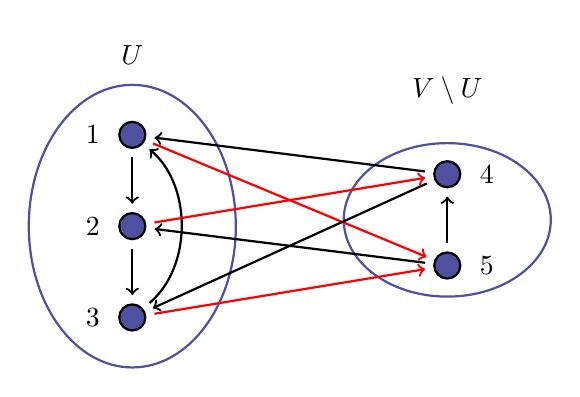
\begin{tikzpicture}[thick,
		  every node/.style={draw,circle},
		  fsnode/.style={fill=myblue},
		  ssnode/.style={fill=myblue},
		  every fit/.style={ellipse,draw,inner sep=-2pt,text width=2cm},
		  ->,shorten >= 3pt,shorten <= 3pt
		]

			% the vertices of U
			\begin{scope}[start chain=going below,node distance=8mm]
			\foreach \i in {1,2,...,3}
			  \node[fsnode,on chain] (f\i) [label=left: \i] {};
			\end{scope}

			% the vertices of V \ U
			\begin{scope}[xshift=4cm,yshift=-0.5cm,start chain=going below,node distance=8mm]
			\foreach \i in {4, 5}
			  \node[ssnode,on chain] (s\i) [label=right: \i] {};
			\end{scope}

			% the set U
			\node [myblue,fit=(f1) (f3),label=above:$U$] {};
			% the set V \ U
			\node [myblue,fit=(s4) (s5),label=above:$V \setminus U$] {};

			% the edges
			\draw (f1) -- (f2);
			\draw (f2) -- (f3);
			\draw (f3) to[out=+40, in=-40] (f1);
			\draw (s5) -- (s4);
			\draw [red] (f1) -- (s5);
			\draw (s4) -- (f1);
			\draw (s5) -- (f2);
			\draw [red] (f2) -- (s4);
			\draw (s4) -- (f3);
			\draw [red] (f3) -- (s5);

		\end{tikzpicture}
	\end{center}
\end{frame}

\begin{frame}{Teorema di Landau}
	\begin{columns}
		\begin{column}{.4 \textwidth}
			\begin{block}{Lemma}
				\begin{equation*}
					\forall v \leq \ell \; \text{ vale } \; \gamma_{n-v} \geq \ell
				\end{equation*}
				\vspace{-3mm}
			\end{block}
		\end{column}
		\begin{column}{.6 \textwidth}

			\begin{gather*}
				\gamma_{n-1} = \ell \\
				\vspace{8mm}
				\gamma_{n-v} - \gamma_{n-v+1} = n - v - s_{n-v+1} \geq \\
				\vspace{8mm}
				n - v - s_n \geq 0 \; \text{ se } \; v \leq \ell
			\end{gather*}
		\end{column}
	\end{columns}

	\begin{center}
		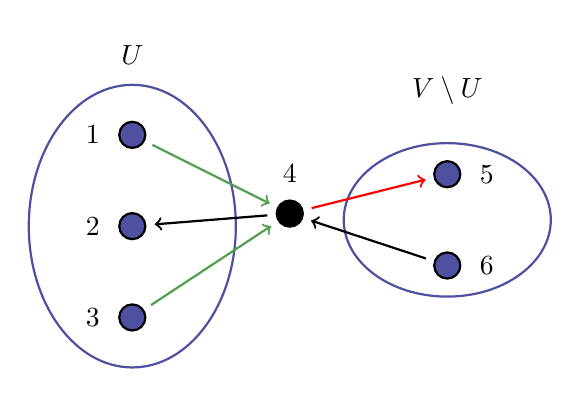
\begin{tikzpicture}[thick,
		  every node/.style={draw,circle},
		  asnode/.style={fill=myblue},
		  bsnode/.style={fill=myblue},
		  csnode/.style={fill=black},
		  every fit/.style={ellipse,draw,inner sep=-2pt,text width=2cm},
		  ->,shorten >= 3pt,shorten <= 3pt
		]

			% the vertices of U
			\begin{scope}[start chain=going below,node distance=8mm]
			\foreach \i in {1,2,...,3}
			  \node[asnode,on chain] (a\i) [label=left: \i] {};
			\end{scope}

			%median Vertex
			\begin{scope}[xshift=2cm,yshift=-1cm,start chain=going below,node distance=8mm]
			  \node[csnode,on chain] (m4) [label=above: 4] {};
			\end{scope}

			% the vertices of V \ U
			\begin{scope}[xshift=4cm,yshift=-0.5cm,start chain=going below,node distance=8mm]
			\foreach \i in {5, 6}
			  \node[bsnode,on chain] (b\i) [label=right: \i] {};
			\end{scope}

			% the set U
			\node [myblue,fit=(a1) (a3),label=above:$U$] {};
			% the set V \ U
			\node [myblue,fit=(b5) (b6),label=above:$V \setminus U$] {};

			% the edges
			\draw [mygreen] (a1) -- (m4);
			\draw [mygreen] (a3) -- (m4);
			\draw (m4) -- (a2);
			\draw [red] (m4) -- (b5);
			\draw (b6) -- (m4);

		\end{tikzpicture}
	\end{center}

\end{frame}

\begin{frame}{Teorema di Landau}
	\begin{block}{Costruiamo induttivamente la matrice di adiacenza}
		$$ j_1 = \min \left\{x \geq 0 \: \big| \: \forall i \geq x,  \; \gamma_i \geq 1 \right\} $$
		$$ j_\delta = \min\left\{x > j_{\delta-1} \: \big| \: \forall i \geq x,  \ \gamma_i \geq \delta \right\} \text{ per } \delta = 2\, , \, \dots \,, \, \ell $$
		\vspace{3mm}
	\end{block}
	\vspace{2mm}
	\pause
	\begin{columns}
		\hspace{8mm} \vspace{5mm}\begin{column}{0.6 \textwidth}
			$\bullet$ $ A_{i, n} = 1 \iff i = j_\delta $ per qualche $\delta$ \\
			\vspace{4mm}
			$\bullet$ $ A_{n, i} = 1 - A_{i, n} $ \\
			\vspace{4mm}
			$\bullet$ $ \sum_{i = 1}^n A_{n, i} = n - 1 - \ell $ \\
			\vspace{4mm}
		\end{column}
		\begin{column}{0.4 \textwidth}
			\[
			\begin{bmatrix}
				0 & 1 & 0 & 0 & \color{red}1 \\
				0 & 0 & 1 & 1 & \color{red}0 \\
				1 & 0 & 0 & 1 & \color{red}0 \\
				1 & 0 & 0 & 0 & \color{red}0 \\
				\color{red}0 & \color{red}1 & \color{red}1 & \color{red}1 & \color{red}0 \\

		    \end{bmatrix}
			\]
		\end{column}
	\end{columns}
\end{frame}

\begin{frame}{Teorema di Landau}
	\begin{block}{Costruiamo induttivamente la matrice di adiacenza}
		$$ j_1 = \min \left\{x \geq 0 \: \big| \: \forall i \geq x,  \; \gamma_i \geq 1 \right\} $$
		$$ j_\delta = \min\left\{x > j_{\delta-1} \: \big| \: \forall i \geq x,  \ \gamma_i \geq \delta \right\} \text{ per } \delta = 2\, , \, \dots \,, \, \ell $$
		\vspace{3mm}
	\end{block}
	\vspace{2mm}
	\begin{columns}
		\begin{column}{0.6 \textwidth}
			\hspace{8mm} $\bullet$ Per costruzione i nuovi $\gamma_k^\prime \geq 0 $ \\
			$$ \sum_{i = 1}^n s_i^\prime = \sum_{i = 1}^n s_i - (n - 1 - \ell) - \ell = $$
			$$ = \binom{n}{2} - (n - 1) = \binom{n-1}{2} $$
			\vspace{8mm}
		\end{column}
		\begin{column}{0.4 \textwidth}
			\[
			\begin{bmatrix}
				0 & 1 & 0 & 0 & \color{red}1 \\
				0 & 0 & 1 & 1 & \color{red}0 \\
				1 & 0 & 0 & 1 & \color{red}0 \\
				1 & 0 & 0 & 0 & \color{red}0 \\
				\color{red}0 & \color{red}1 & \color{red}1 & \color{red}1 & \color{red}0 \\

		    \end{bmatrix}
			\]
		\end{column}
	\end{columns}
\end{frame}

\begin{frame}{Complessità: Dimostrazione}
	\begin{block}{Calcolo dei Momenti}
		Sia $x \in V$ con $k = d^-(x)$ e $\phi_n^k$ il numero di lookup sulla riga di $x$, allora
		$$ \mathbb{E}\left[\phi_n^k\right] = O\left(\frac{n\ell}{k}\right) $$
		$$ \mathbb{E}\left[\left({\phi_n^k}\right)^2\right] = O\left(\frac{n^2\ell^2}{k^2}\right) $$
		E la costante moltiplicativa è uniforme in $k$.
	\end{block}
\end{frame}

\begin{frame}{Calcolo dei Momenti}
	%Pongo $ E^k_n = \mathbb{E}\left[\phi_n^k\right] $ allora
	\begin{block}{Idea}
		La distribuzine uniforme su $\mathcal{S}_{n+1}$ si ottiene da quella di $\mathcal{S}_n$ inserendo $n+1$ con probabilità uniforme.
	\end{block}
	\begin{equation*}
		\mathbb{E}\left[\phi_{j+1}^k\right] = \sum_{i=1}^j \mathrm{P}\left(\phi_j^k = i\right) \left(i + \frac{i}{j+1}\right)
	\end{equation*}
	\vspace{4mm}
	\pause
	$$ \begin{cases}
		\mathbb{E}\left[\phi_k^k\right] = \ell  \\
		 \mathbb{E}\left[\phi_{j+1}^k\right] = \frac{j + 2}{j + 1}\,\mathbb{E}\left[\phi_j^k\right]  \\
	\end{cases} \implies \mathbb{E}\left[\phi_n^k\right]  = \frac{n+1}{k+1}\ell $$



\end{frame}

\begin{frame}{Calcolo dei Momenti}
	\begin{allign*}
	\begin{equation*}
		\mathbb{E}\left[\left({\phi_{j+1}^k}\right)^2\right] = \sum_{i=1}^j \mathrm{P}\left(\phi_j^k = i\right) \left(i^2 + \frac{i}{j+1}\left(2i + 1\right)\right) =
	\end{equation*}
	\begin{equation*}
		\hspace{2.5cm}= \left(1 + \frac{2}{j + 1}\right)\mathbb{E}\left[\left({\phi_j^k}\right)^2\right] + \frac{1}{j + 1} \mathbb{E}\left[\phi_j^k\right] =
	\end{equation*}
	\begin{equation*}
		\hspace{-0.2cm} = \, \frac{j + 3}{j + 1}\mathbb{E}\left[\left({\phi_j^k}\right)^2\right] + \frac{\ell}{k + 1}
	\end{equation*}
	\end{allign*}

	\vspace{4mm}
	$$ \text{Inoltre } \mathbb{E}\left[\left({\phi_k^k}\right)^2\right] = \ell^2 $$

\end{frame}

\begin{frame}{Calcolo dei Momenti}
	\begin{equation*}
		\mathbb{E}\left[\left({\phi_{j+1}^k}\right)^2\right] = \frac{\left(n+1\right)\left(n+2\right)}{\left(k+1\right)\left(k+2\right)} \ell^2 + \frac{\ell}{k+1} \sum_{w=k}^n \frac{\left(n+1\right)\left(n+2\right)}{\left(w+1\right)\left(w+2\right)} =
	\end{equation*}
	\begin{equation*}
		= O\left(\frac{n^2\ell^2}{k^2}\right) + O\left(\frac{n^2\ell}{k^3}\right) = O\left(\frac{n^2\ell^2}{k^2}\right)
	\end{equation*}
\end{frame}

\begin{frame}{Complessità: Dimostrazione}
	Il numero di lookup è
	\begin{equation*}
		\tilde\xi = \sum_{2^j \leq n} \xi_j
	\end{equation*}
	\begin{equation*}
		\xi_j \; = \sum_{x \in V_j \setminus V_{j+1}} \phi_x\,, \; \;
		V_j = \left\{x \in V \, \bigg| \, d^-(x) \leq \ \frac{n}{2^j}\right\}
	\end{equation*}

	\pause
	\begin{block}{Calcolo di $|V_j|$}
		\begin{equation*}
			d^-(x_1) \leq  \dots \leq d^-(x_n) \implies k \, d^-(x_k) \geq \sum_{i=1}^k d^-(x_i) \geq \binom{k}{2}
		\end{equation*}
		\begin{equation*}
			k \, \leq \, 2 d^-(x_k) + 1 \implies |V_j|  \, \leq \, \frac{n}{2^{j-1}} + 1
		\end{equation*}
	\end{block}
\end{frame}

\begin{frame}{Complessità: Dimostrazione}
	\begin{equation*}
		\mathbb{E}\left[\xi_j\right] = \sum_{x \in V_j \setminus V_{j-1}} \mathbb{E}\left[\phi_{n}^{n/{2^j}}\right] \leq \left(\frac{n}{2^{j-1}}+1\right) \frac{n}{{n}/{2^{j+1}}} \leq 8 \, \ell n
	\end{equation*}
	\vspace{2mm}
	\pause
	\begin{equation*}
		\mathbb{E}\left[\xi_j^2\right] = \sum_{x \in V_j \setminus V_{j-1}} \mathbb{E}\left[\left(\phi_{n}^{n/{2^j}}\right)^2\right] \leq \left(\frac{n}{2^{j-1}}+1\right) \frac{n^2}{\left({n}/{2^{j+1}}\right)^2} \leq 8 \, \ell^2 n \, 2^j
	\end{equation*}
	\vspace{2mm}
	\pause
	\begin{equation*}
		\mathbb{E}\left[\tilde\xi\right] = \sum_{2^j \leq n} \mathbb{E}\left[\xi_j\right] = O\left(\ell n \log\left(n\right)\right)
	\end{equation*}
	\vspace{2mm}
	\begin{equation*}
		\mathbb{E}\left[{\tilde\xi}^2\right] = \sum_{2^j \leq n} \mathbb{E}\left[{\xi_j}^2\right] = O\left(\ell^2 n^2\right)
	\end{equation*}
\end{frame}

\begin{frame}{Complessità: Dimostrazione}
	\begin{block}{Stima con Alta Probabilità}
		\begin{equation*}
			\mathrm{P} \left(\tilde\xi > \mathbb{E}\left[\tilde\xi\right] + \ell n \log(n)\right) \leq \frac{\mathrm{Var}\left[\tilde\xi\right]}{\left(\ell n \log(n)\right)^2} = O\left(\frac{1}{{\log(n)}^2}\right)
		\end{equation*}
	\end{block}
	\begin{block}{Improvement}
		Utilizzando una stima esponenziale sulla convergenza della somma di v.a. i.i.d. (\textit{Chernoff Bound}) si può ottenere una stima più forte, ovvero

		$$ O\left(\frac{1}{n}\right) $$

	\end{block}
\end{frame}

\begin{frame}{Bibliografia}
	\begin{itemize}
		\item $\bullet$ Alfred Brauer, Ivey C. Gentry, and Kay Shaw \textit{A New Proof of a Theorem by H. G. Landau on
			Tournament Matrices} Journal of Combinatorial Theory 5, 289--292 (1968)
		\vspace{4mm}
		\item $\bullet$ Gregory Gutin, George B. Mertzios and Felix Reidl \textit{Searching for Maximum Out-Degree
			Vertices in Tournaments} arXiv:1801.04702 [cs.DS]

	\end{itemize}

\end{frame}

\end{document}
